\chapter{Appendix}
\section{Projects that have been already built upon Anacleto:}
\subsection{W7X - trigger }
\cite{RIGONI2018122}
The Anacleto framework has been used to develop a general purpose timing device to be used in Wendelstein 7-X diagnostics. The timing device is implemented in a Red Pitaya board and defines two digital outputs to generate clock and gate signals, and two digital inputs to receive a synchronizing 10 MHz clock and a trigger signal. The board is configured via software to generate a pre-programmed timing sequence after the system has been armed and a trigger input signal has been received. The timing sequence is communicated via TCP/IP to the ARM processor hosted in the Zynq chip of the Red Pitaya board. In this case a set of registers have been defined as interface between the processor and the FPGA application, without using interrupt lines. All registers except one are used to specify the time sequence. The remaining register is used as command register to arm and disarm the board. Not considering the time required for developing the FPGA application written in VHDL the creation of the new project, the adaption of the driver from the template and the deploy required less than one working day.

\begin{figure}
    \centering
    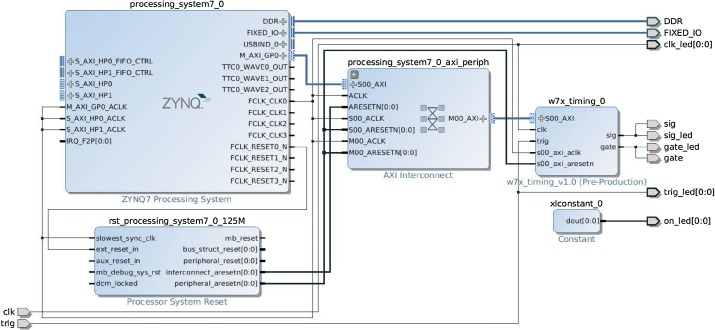
\includegraphics{img/APPENDIX/W7X_VHDL.jpg}
    \caption{A sketch of the overall organization in the VHDL component provided by Vivado Xilinx Tool showing the interconnection between the Zynq processing unit and the custom logic that perform the timing. }
    \label{fig:W7X}
\end{figure}


\subsection{fast event driven data acquisition for the NIO negative ion beam}
~
A desired topics for a DAQ device is the possibility to increase the level of detail during acquisition based on particular events. It is not uncommon to have an observed quantity that changes rapidly in time and than last steady or possibly in a non interesting state for long periods. An example of is the breakdown event that occurs in the accelerator grids of a ion source, leading to a very fast transient change in the measured currents and voltages of the grid power supply. In this case, fast data acquisition must be triggered by the event itself, acquiring data for a short time window around the event occurrence. This technique has been applied to Nio experiment~\cite{DEMURI2015249} a small radio frequency negative ions beam source with a high voltage electrostatic particle accelerator stage composed of grids. In certain conditions break-down events~\cite{RECCHIA20111545} appear on the high voltage gaps of the grids causing a  high current discharges of the power supply feeding the accelerator. 
~
A subset of the FPGA functionality described in section 3 has been implemented in a Red Pitaya device, namely the trigger logic to detect the occurrence of the event, the pre and post trigger sampling logic and the FIFO/DMA data transfer to computer memory via the GNU Linux driver. In this case data are streamed and when an event is detected and data collected at 5 MHz sampling speed along the corresponding time window, the data block is passed, either via FIFO or DMA, to the linux driver and then, in turn, to a program in the Zynq processor that communicates the newly acquired data block to the central data acquisition system via TCP/IP. The results are displayed in Fig. 4, showing the events acquired during a beam generation lasting 2 hours. Each time window lasts 1 ms, and one enlarged event is  displayed in the lower part of Fig. 4.    
\begin{figure}
\centering
%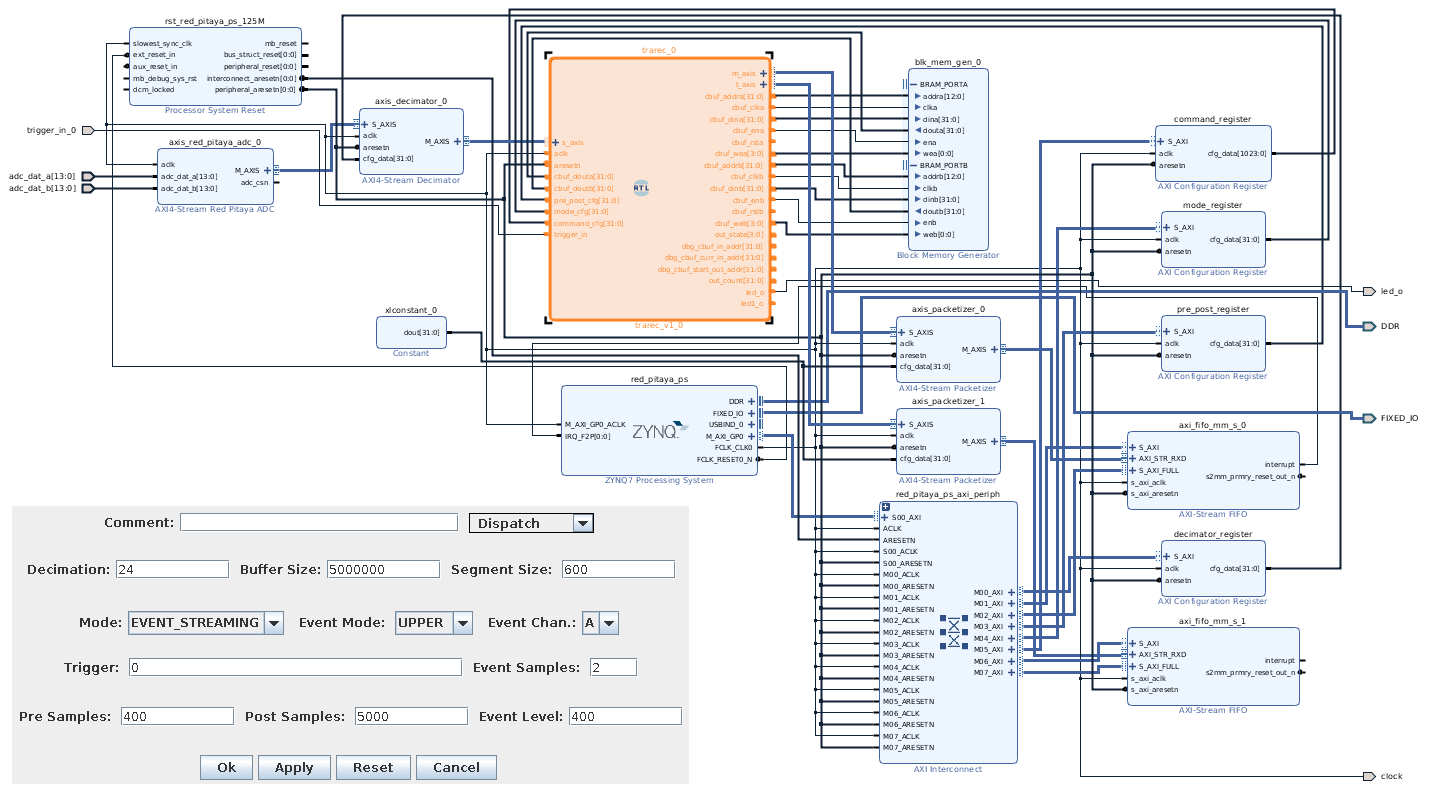
\includegraphics[width=0.59\textwidth]{img/nio_scm1.png}
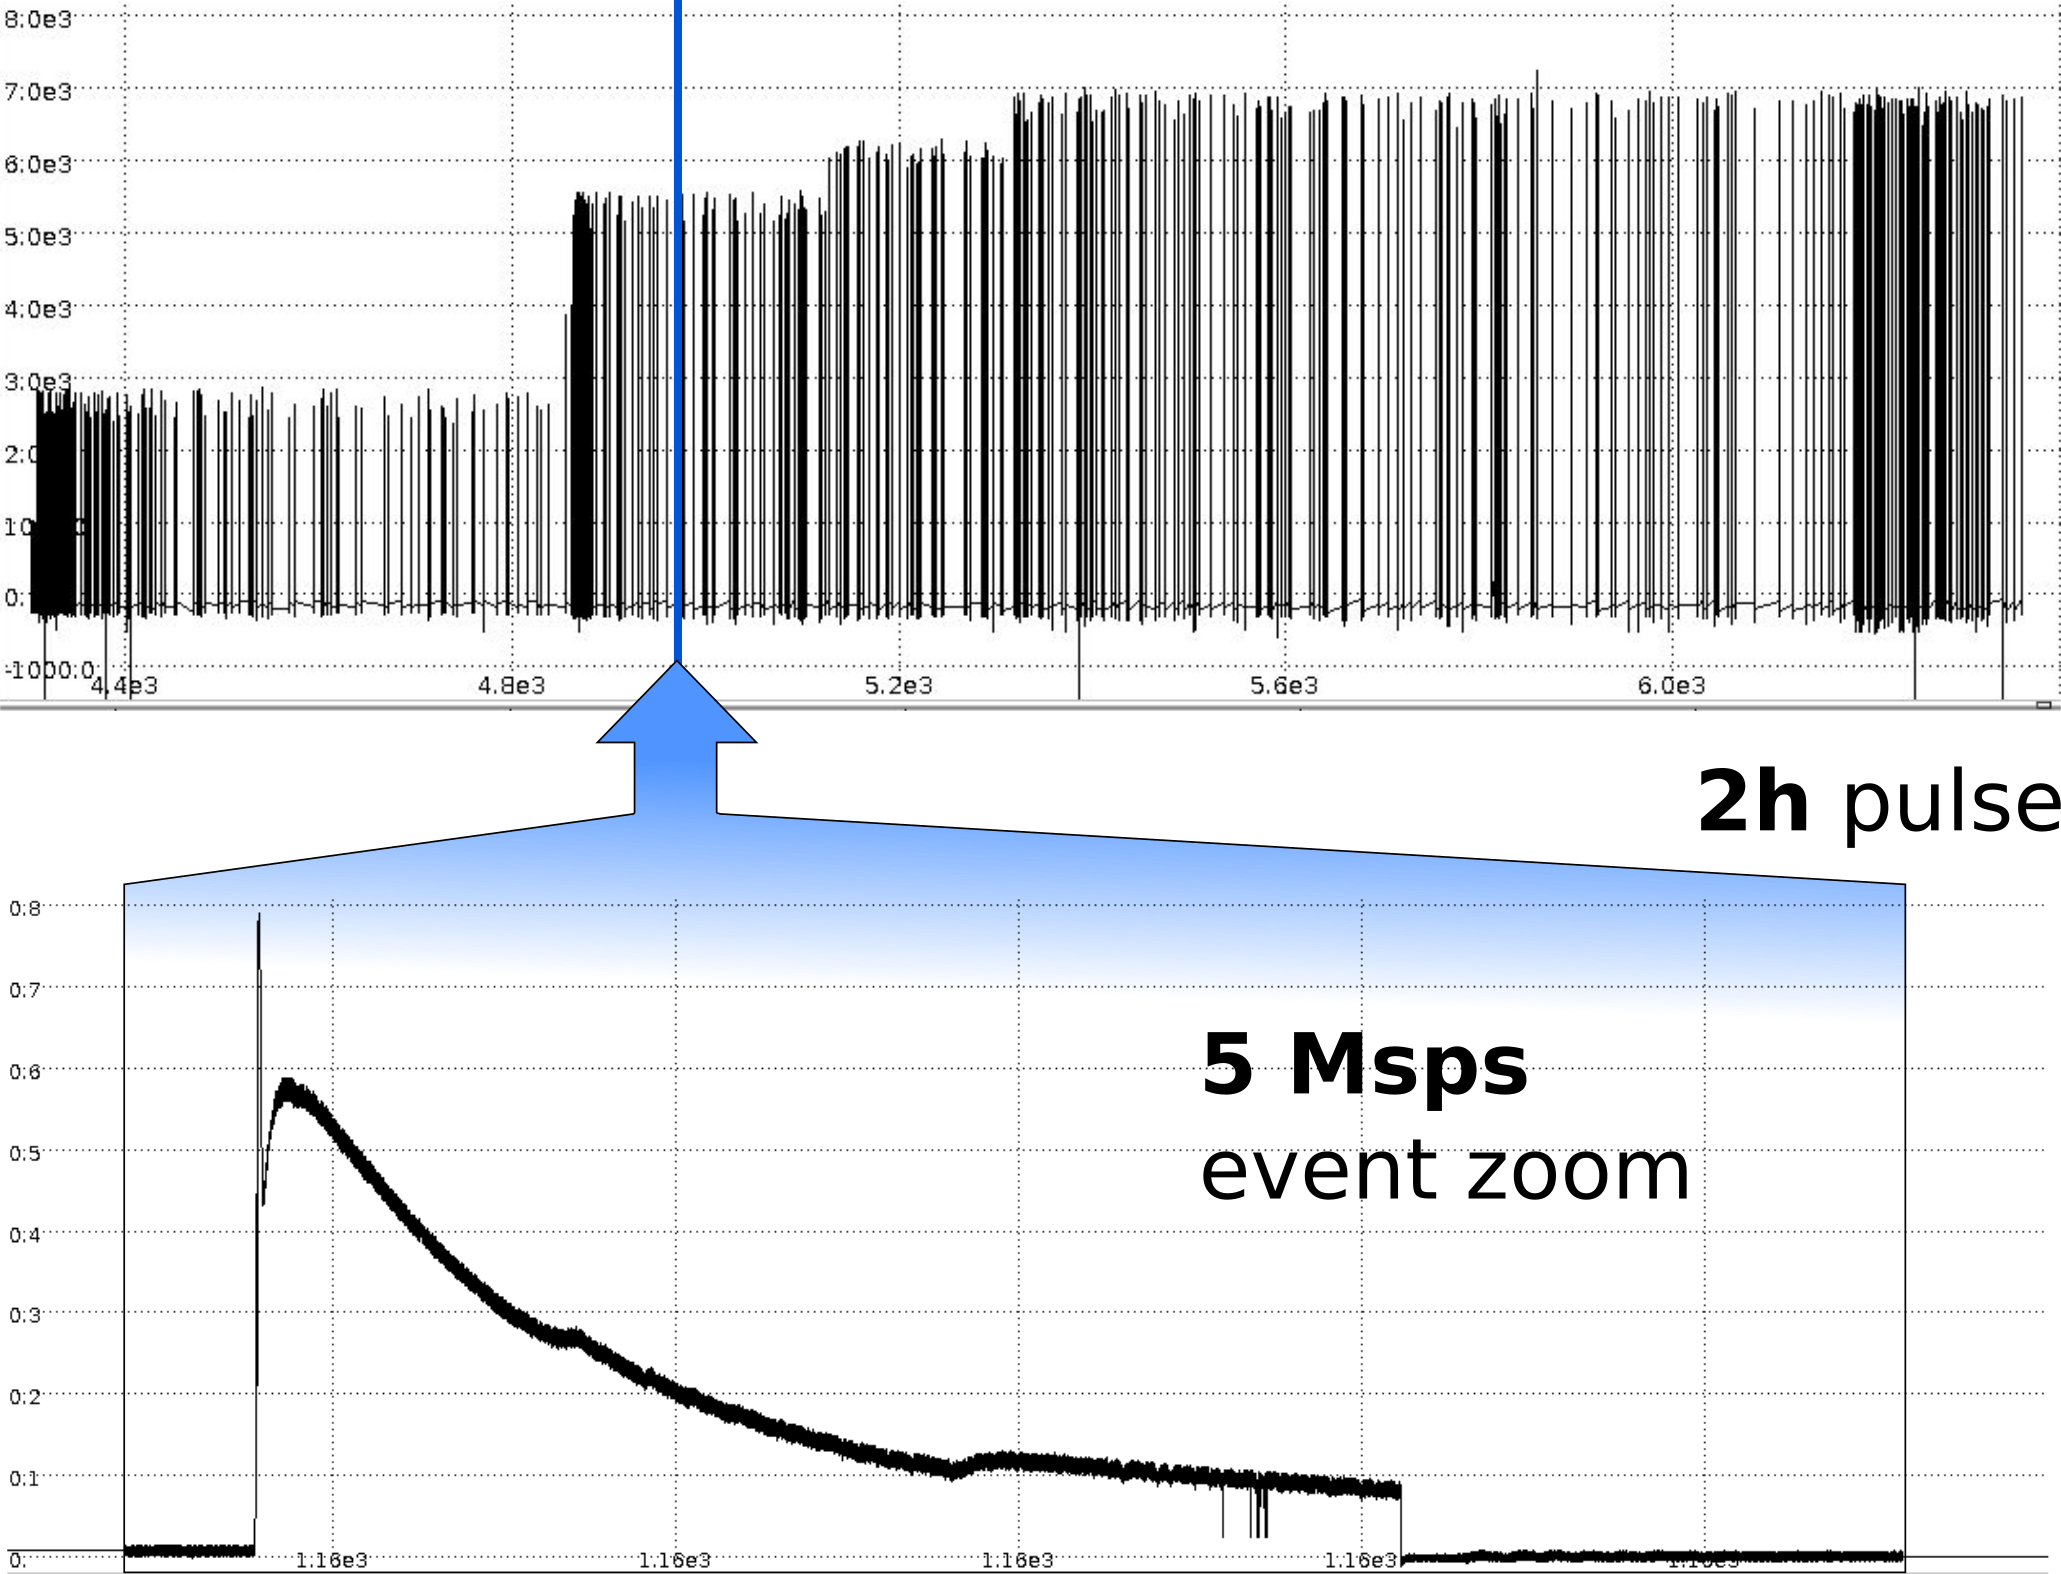
\includegraphics[width=0.49\textwidth]{img/4_EmbeddedML/nio12b.png}
\caption{Figure example.}
\label{fig:nio}
\end{figure}


\subsection{STRIKE beamlets indentification}

The instrumented calorimeter STRIKE (Short-Time Retractable Instrumented Kalorimeter Experiment) has been designed to work with the characterization of the negative ion beam in terms of beam uniformity and divergence during short pulse operations. STRIKE is made of 16 1D Composite Carbon Fiber (CFC) tiles, intercepting the whole beam and observed on the rear side by infrared (IR) cameras.
The beamlet parameters, such as dimension, divergence, position and amplitude, For this purpose to convolutional neural network, CNN, is trained to detect the beamlets and their features on the images from IR. As STRIKE just started to operate, the training was performed with artificial data built on purpose.

\subsubsection{Strike beamlet heat deploy}
The STRIKE calorimeter has been specifically designed with the purpose of characterizing the negative ion beam in terms of beam uniformity and divergence during short pulse operations. All 1280 beamlets coming from the SPIDER extraction and acceleration grids are deployed in STRIKE divided into 16 1D Carbon Fiber Composite (CFC) tiles that can be observed on the rear side by infrared (IR) cameras [1]. The front observation presents some drawbacks two to the background noise caused by: the optically emitting gas between the beam source and the calorimeter, and the material sublimated from the calorimeter surfaces two to the heating itself.
Being a well-known ill-posed problem, it includes finite element code to solve the direct problem. Anyway that is not applicable to STRIKE operation, being a high machine time consuming. 

The whole identification system can be divided in two steps named Jasper and Horace. Jasper is the part deputed to the flux reconstruction, while Horace is the software component responsible for the identification of beamlets parameters.

Horace is meant to be applied to the reconstructed images of the heat deposition produced by Jasper so it considers STRIKE completely transparent to the heat flux model of the tiles. Even if they do not know almost anything about each other, Jasper and Horace share the same greedy approach of NN implementation. 
The inversion of the whole model was such decomposed in these two subsequent steps because of the different nature of the two associated phenomena themselves. Indeed from the Jasper point of view we are looking for STRIKE non-stationary heat transfer parameters, whereas we are considering to relate directly with the physical model of the extraction of the beamlets in Horace. For this reason, although they both exploit a NN approach, the two implementations are very different.

\subsubsection{Horace}
As said before, Horace is the software component responsible for the identification of the beamlets parameters and it is meant to be applied to the reconstructed images of the heat deposition produced by Jasper. Horace considers the input image as the direct displacement and shape of the beamlets themselves, so takes as input an image of the reconstructed heat deposition on STRIKE and produces as output a set of numerical parameters for each of the beams.
The proposed implementation relies on a CNN ( Convolutional Neural Network ) where the activation of the output nodes are directly representing the desired numerical values for the parameters. 
CNNs have recently become the method of choice for processing visual and other two-dimensional data. They have proven to be very effective in areas such as image recognition and classification; they have been successful in identifying faces, objects and traffic signs apart from powering vision in robots and self driving cars.
CNNs were inspired by biological processes in that the connectivity pattern between neurons resembles the organization of the animal visual cortex. Individual cortical neurons respond to stimuli only in a restricted region of the visual field known as the receptive field. The receptive fields of different neurons partially overlap such that they cover the entire visual field.
CNNs use relatively little pre-processing compared to other image classification algorithms. This means that the network learns the filters that in traditional algorithms were hand-engineered. This independence from prior knowledge and human effort in feature design is a major advantage. 
Not only are CNN able to identify objects but also other features like their position, color or dimension. 
So, the network has been thought to be space partitioned, see Figure x, in the sense that the all beamlets image plane is divided in a grid and a small size network is applied for each of the grid space. We are assuming that the total reconstructible number of objects per subspace is limited by the fact that it very unlikely that many bemlets will insist to the same point at the same time, and also that this unfavorable situation should never happen in a real scenario because it must be stopped before. 
\begin{figure}
    \centering
    \subfigure[]{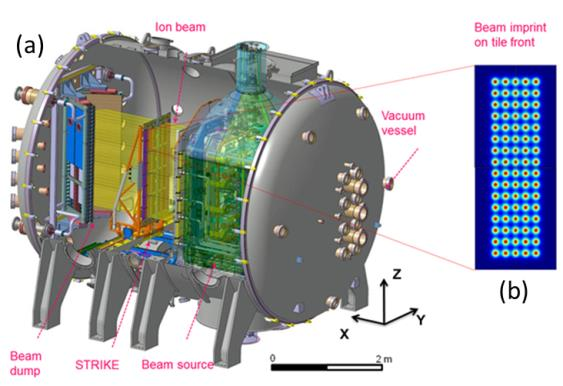
\includegraphics[height=4cm]{img/APPENDIX/HORACE/image3.png} \label{fig:strike_a}}
    \subfigure[]{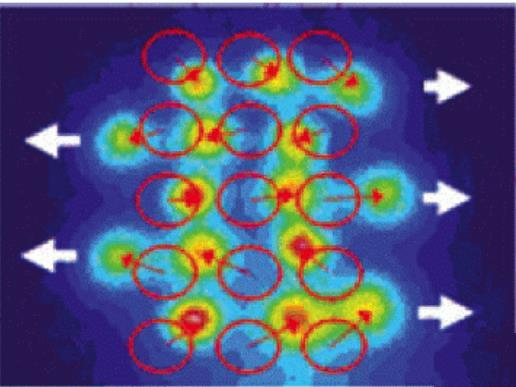
\includegraphics[height=4cm]{img/APPENDIX/HORACE/image7.jpg} \label{fig:strike_b}}
    \caption{A drawing of SPIDER experiment and the STRIKE component, with a simulation of beamlets deposition on a tile (a), and a computer aided simulation of the possible drift effect that may corrupt the impact position of the beamlets (b).}
    \label{fig:strike}
\end{figure}
The \Figure{\ref{fig:horace_net}} describes the layers organization of a single subspace network, where the input image was set to be a monochrome 200x300 pixels map with 8 bit values. The image feeds into the network composed by a set of convolutional layers and a subsequent network of standard feed forward relu activated nodes. The typical parameters for the convolution layer in a CNN are: the amount of nodes involved, the size of the convolution kernel and the stride. The former convolutional portion is composed in this case by 128 nodes with 10x10 pixels kernel and stride 2. A further operation can be also applied between two subsequent convolutions gradually to reduce the dimensionality (usually a max-pooling).
\begin{figure}
    \centering
    
\includegraphics[height=6cm]{img/APPENDIX/HORACE/image2.png}
    \caption{A sketch of the deep convolutional network exploited by Horace to indentify position and size of the beamlets projected on STRIKE tiles.}
    \label{fig:horace_net}
\end{figure}
For this very early test campaign the Horace network has been trained with a simulated model that generates bivariate gaussian-shaped images, one per each of the desired beamlet in the subspace. For the generation of the gaussians images we used the standard multivariate formulation of the gaussian distribution:
\begin{equation}
    f_{\bm{X}}(x_1, ... ,x_k) = 
    \frac{\exp{\left( -\frac{1}{2}\transpose{(\bm{x}-\mu)} \Sigma^{-1} (\bm{x}-\mu) \right)}}
         {\sqrt{(2\pi)^k |\Sigma|}}
\end{equation}

where we obtained the covariance matrix by linear combination of the beamlet spread along its main axes and a rotation operator
\begin{equation}
    \Sigma_R = R SS R^{-1}   \hspace{3cm}   S=\transpose{[\lambda_1,\lambda_2]}\mathbb{I}
\end{equation}
Where the standard deviations along axes and rotation are the sx, sy and rot labels of the network outputs.

Once we will validate the model inversion functionality in the simple case of the subspace for the foreseen maximum number of gaussians that will insist upon the same subspace, a further parameter will be added to represent the confidence level of the beamlet identification, likewise the multi-class identification in YOLO networks~\cite{YOLOv3} where the confidence level is used to discriminate the presence of a particular object in space. Here the difference is that we do not have different classes of object but the same object (gaussian 2D spot) with different parameters.

\begin{figure}
    \centering
    \subfigure[]{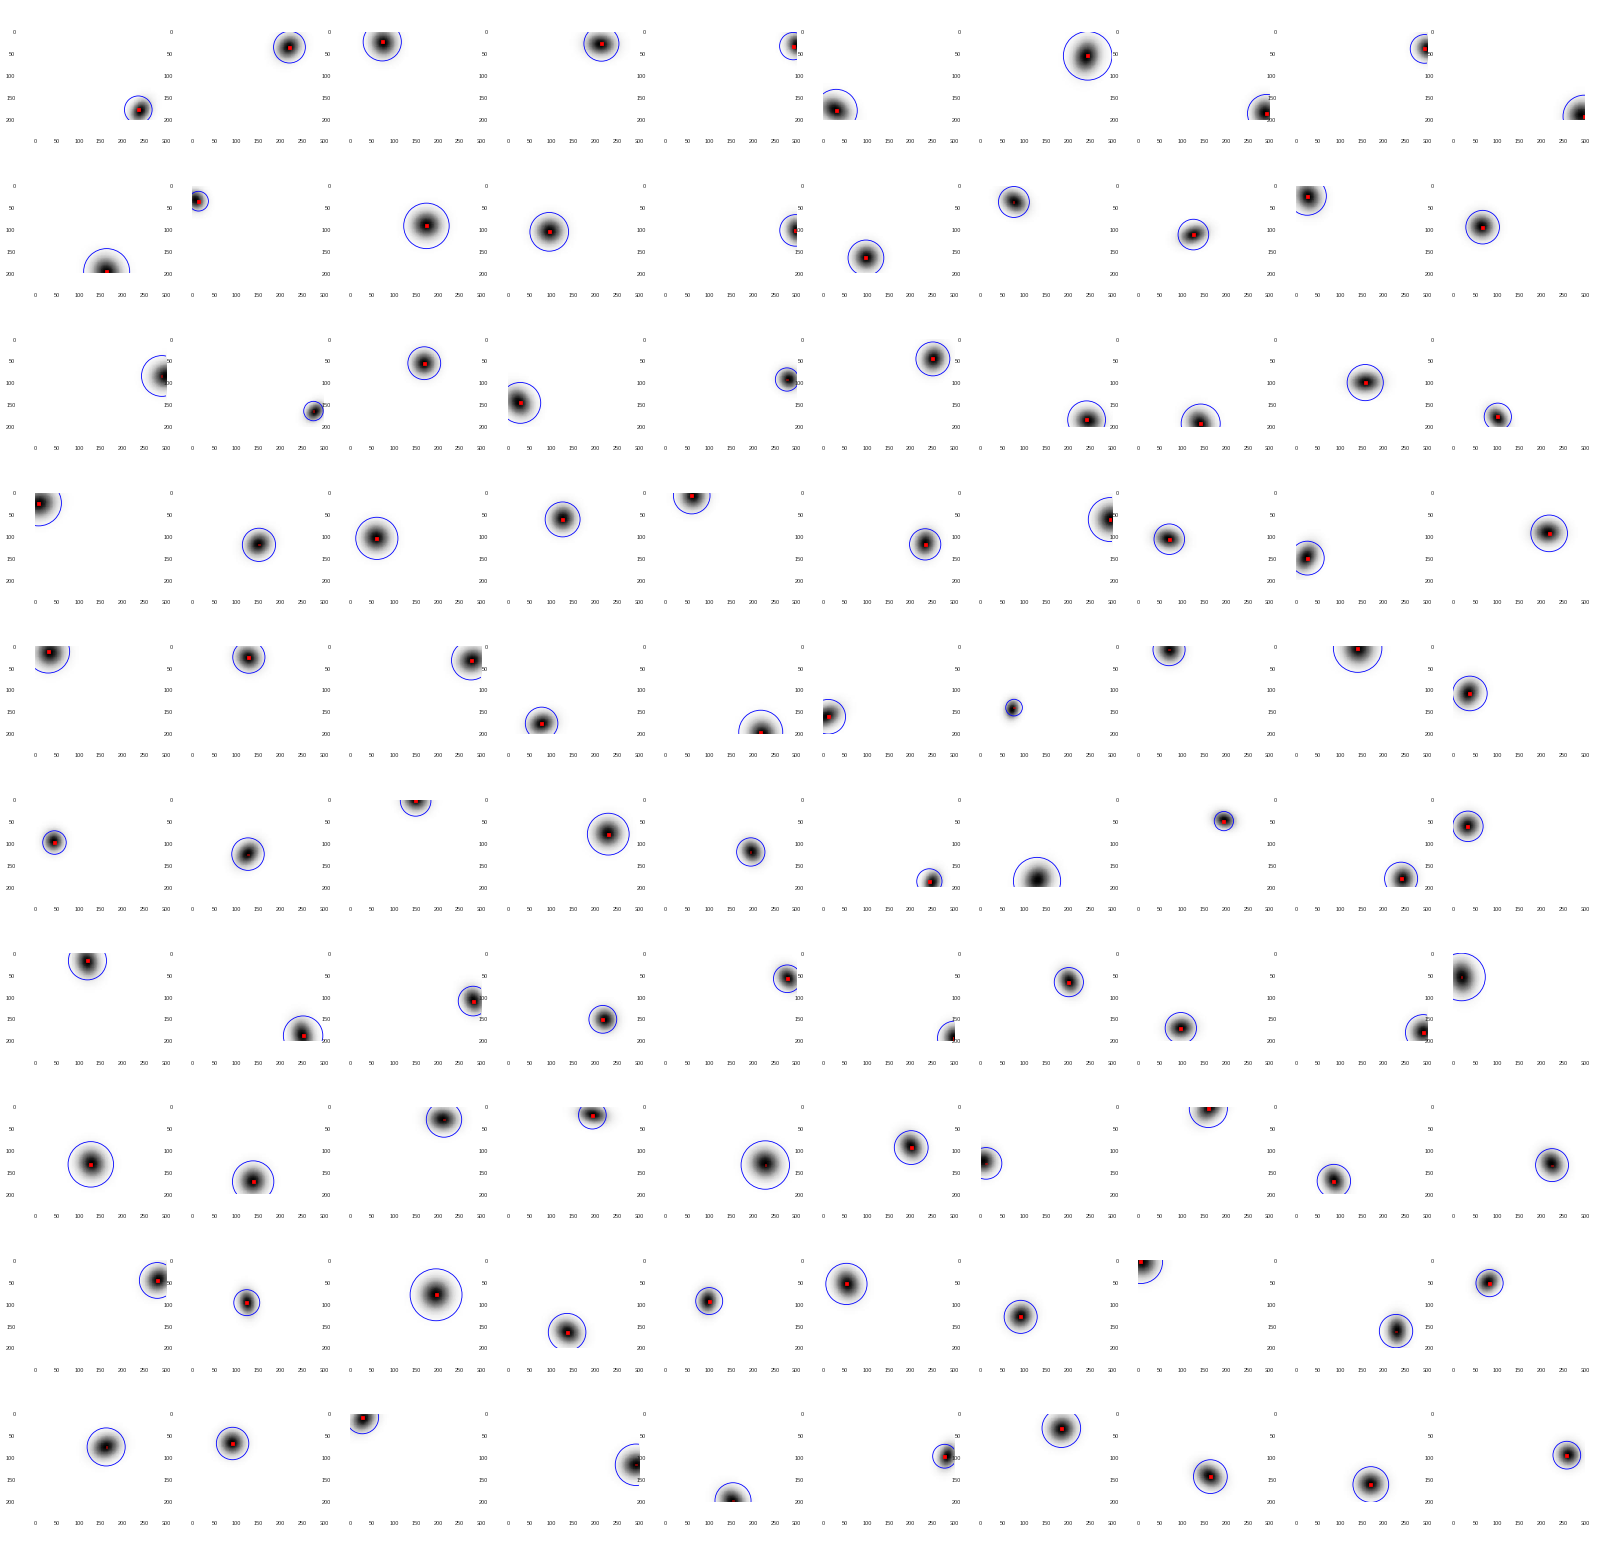
\includegraphics[width=10cm]{img/APPENDIX/HORACE/image1.png} \label{fig:horace_spots_a}}
    \subfigure[]{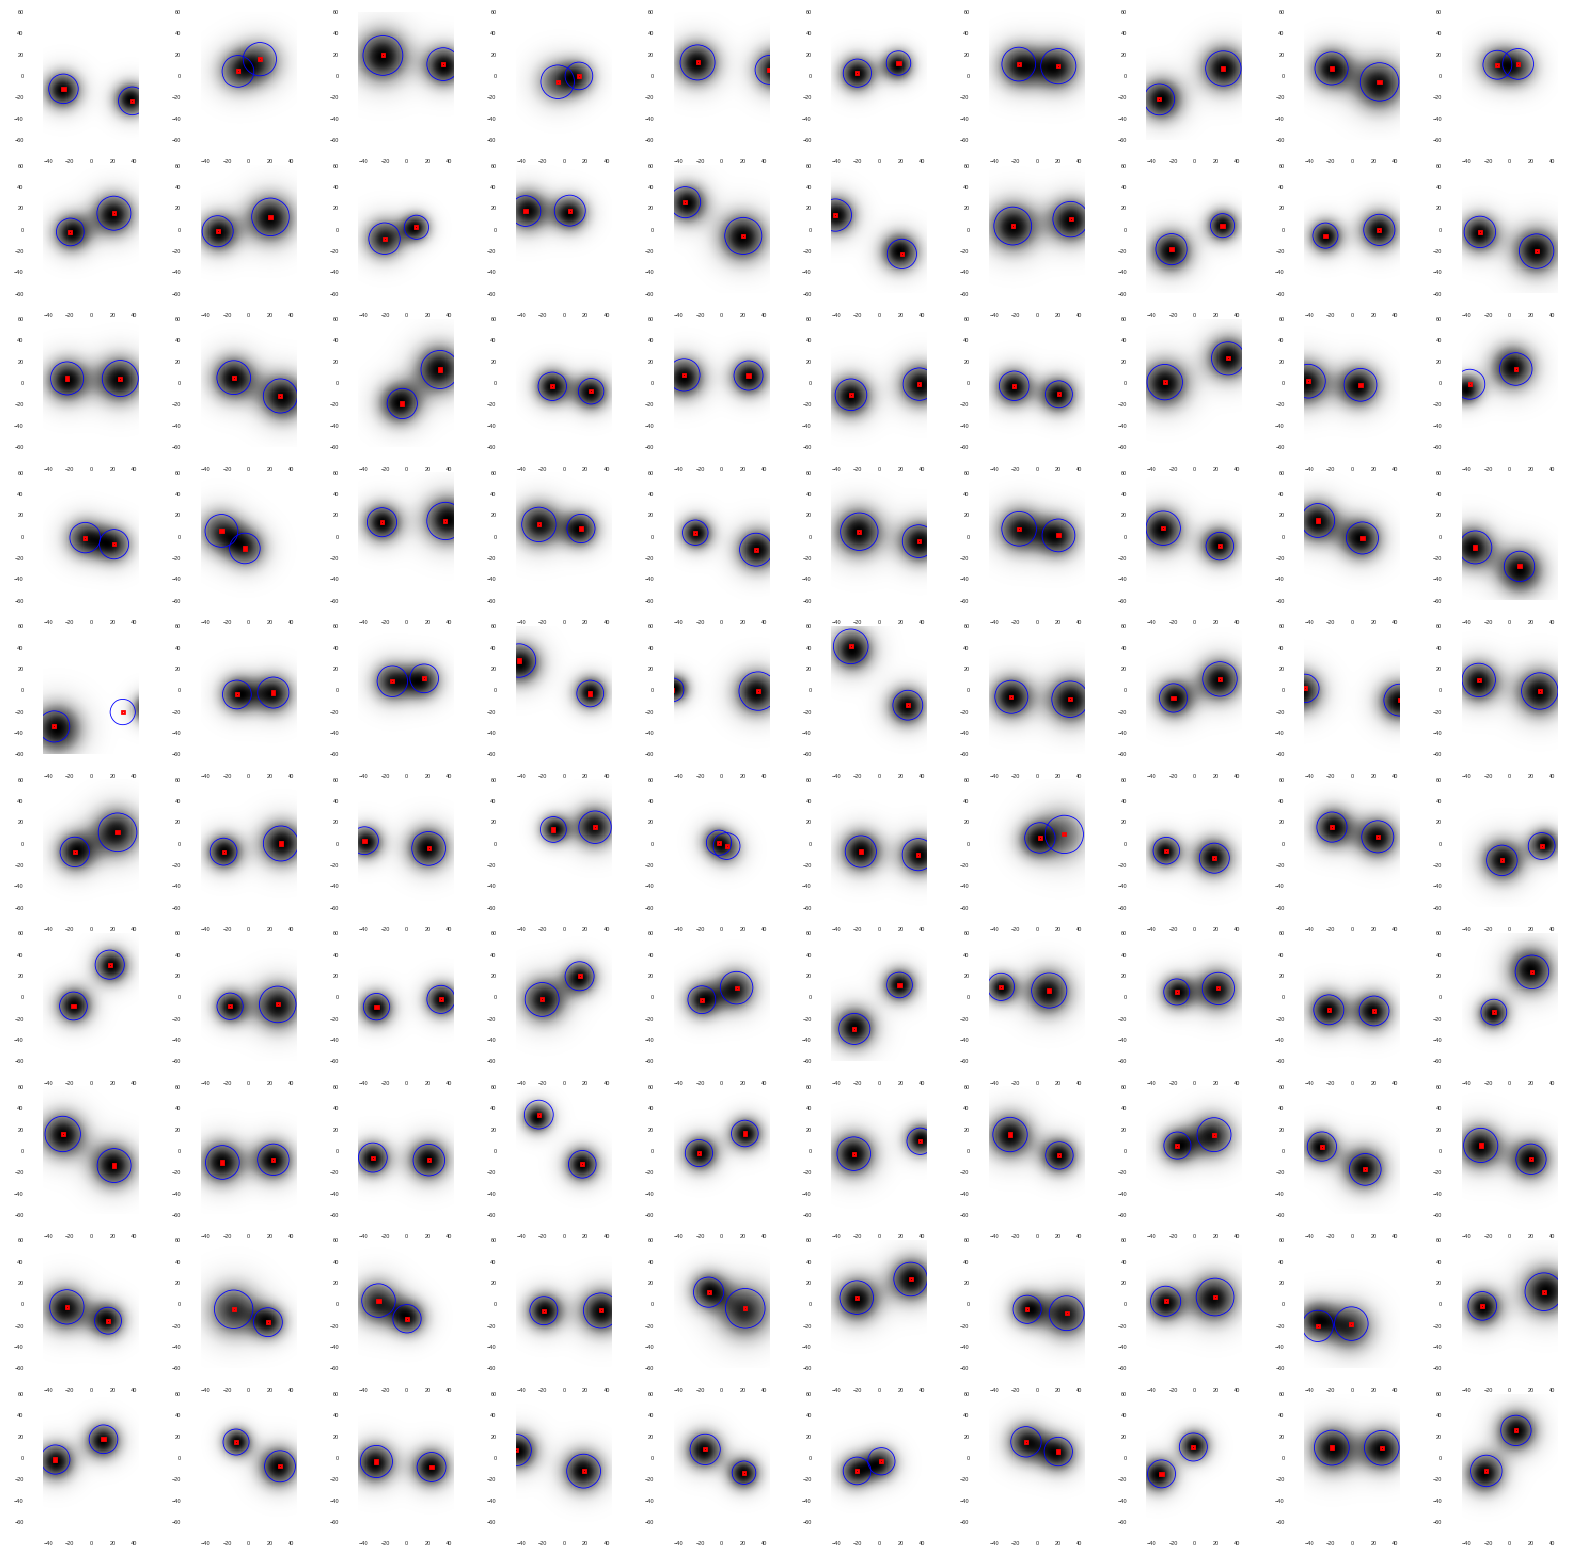
\includegraphics[width=10cm]{img/APPENDIX/HORACE/image9.png} \label{fig:horace_spots_b}}
    \caption{Two batches visualization of Horace identifications for single beamlet (a) and double beamlet (b). }
    \label{fig:horace_spots}
\end{figure}